% Chapter 6 draft (2026-11-01). Drop-in replacement for the current Chapter 6 of
% Sally_Sun_Honours_Thesis_4.pdf. Needs: booktabs, graphicx, xcolor, amsmath.
% Source of every number: notes/thesis/chapter6_sources.md (which probe, which CSV, which note).
% \pending{...} marks text that waits on a run that has not been done; delete each once filled.
\providecommand{\pending}[1]{\textcolor{red}{[#1]}}

\chapter{Simulation Study}
\label{ch:simulation}

This chapter tests the methods of Chapters~4 and~5 on simulated streams whose true dependence is
known at every tick. Section~\ref{sec:design} sets out the design. Section~\ref{sec:fixed} measures
how the error of a fixed forgetting factor depends on memory, which is the trade-off of
Section~5.1. Section~\ref{sec:adaptive} compares the two ways of choosing memory online: the bank
of Algorithm~1 and a variable forgetting factor. Section~\ref{sec:loss} asks which loss the bank
should score with. Section~\ref{sec:shape} turns to changes in the shape of the copula that leave
Spearman's $\rho_S$ unchanged, and to tail dependence. Section~\ref{sec:cost} reports storage and
time per tick, and Section~\ref{sec:summary} summarises.

% -----------------------------------------------------------------------------
\section{Experimental design}
\label{sec:design}

\subsection{Data-generating process}

Each simulated stream is a sequence of pairs $(X_t,Y_t)$, $t=1,\dots,N$, drawn independently
across $t$ given a deterministic dependence path. At tick $t$ a scalar $d_t\in(-1,1)$ fixes a
target Spearman's rho,
\[
  \rho_{S,t}=\frac{6}{\pi}\arcsin\!\left(\frac{d_t}{2}\right),
\]
which is the Spearman's rho of a Gaussian copula with correlation $d_t$. A copula family is then
parametrised to have exactly this $\rho_{S,t}$, by inverting the family's
$\rho_S(\theta)$ relation of Section~3.2, and a pair $(U_t,V_t)$ is drawn from it. The observations
are the normal scores $X_t=\Phi^{-1}(U_t)$ and $Y_t=\Phi^{-1}(V_t)$, so both margins are standard
normal and stationary in every scenario. Four families are used: Gaussian, Clayton, Gumbel and
Student~$t$ with $\nu=4$. Because the families are matched on $\rho_S$, any difference between
them in an experiment is a difference in the shape of the copula, mainly in its tails, and not in
the overall strength of association. Clayton and Gumbel cannot represent negative dependence; for
a negative target their parameter is held at the independence boundary, so their true $\rho_S$ is
approximately zero there.

The ground truth for each tick is the achieved $\rho_{S,t}$ of the copula actually sampled. For
the log-score metric it is the true copula density $c_t(u,v)$, evaluated at the true
probability integral transform $(U_t,V_t)$.

Two consequences of this design matter for interpreting the results. First, since the margins are
known and stationary, any marginal estimation error comes only from the finite rank window of
Section~\ref{sec:estimators}; with real data the margins would also drift. Second, given the
dependence path the observations are independent, so the assumption
$\mathbb E[\hat p_t\mid\mathcal F_{t-1}]\approx\rho_{S,t}$ used in Section~5.3.1 holds up to the
$O(1/W)$ bias of the rank pseudo-observations.

The live server of Section~2.3 uses the same copula sampler, so a live stream and an offline
stream with the same scenario are draws from the same process. The live server additionally turns
the normal scores into geometric Brownian motion prices; that step is a deterministic, monotone
transform of each margin and so does not change the copula.

\subsection{Scenarios}

Each stream has $N=5000$ ticks. The first 500 are a burn-in and are not scored. The four
dependence paths are listed in Table~\ref{tab:scenarios}.

\begin{table}[ht]
  \centering
  \caption{Dependence scenarios. $\rho_S$ is the Gaussian-family value; for Clayton and Gumbel,
    negative targets are replaced by approximately $0$.}
  \label{tab:scenarios}
  \begin{tabular}{lll}
    \toprule
    Scenario & Path of $d_t$ & True $\rho_{S,t}$ \\
    \midrule
    constant  & $d_t=0.6$ & $0.582$ throughout \\
    drift     & linear from $-0.5$ to $0.8$ over $t=0,\dots,N$ & $-0.482\to0.786$ \\
    jump      & $0.2$ for $t<2500$, then $0.8$ & $0.191\to0.786$ at $t=2500$ \\
    oscillate & $0.6\sin(2\pi t/400)$ & between $\pm0.582$, period 400 ticks \\
    \bottomrule
  \end{tabular}
\end{table}

The scenarios are chosen so that the memory that minimises error is different in each:
\emph{constant} rewards the longest memory available, \emph{oscillate} the shortest, and
\emph{drift} something in between. \emph{jump} rewards long memory before the change and short
memory just after it, so no fixed memory is right for the whole run.

\subsection{Estimators and forgetting}
\label{sec:estimators}

Three online estimators of $\rho_S$ are compared, each with exponential forgetting at weight
$\lambda$ on the newest observation (the convention of Section~5.1):
\begin{itemize}
  \item the forgetting empirical-copula estimator of Section~4.2.2 (``Xiao''), with a
    $20\times20$ grid;
  \item the Hermite series estimator of Section~4.2.3, with order $N=10$;
  \item online maximum pseudo-likelihood (MPL) for a Gaussian copula, Section~4.3.2, with
    expected Fisher scoring in the coordinate $\operatorname{atanh}\rho$ (Section~3.5.4).
\end{itemize}
Memory is reported throughout as the number of ticks $M$, related to the forgetting weight by
$\lambda=2/(M+1)$; for an exponential filter $M$ is also the steady-state effective sample size.
Inside the bank and the variable-forgetting comparisons, all three estimators receive the same
pseudo-observations: the ranks $\hat U_t,\hat V_t$ of $X_t,Y_t$ among the previous $W=500$
observations, computed as $R/(W+2)$ before $X_t,Y_t$ are added to the window, and passed to the
estimators as normal scores $\Phi^{-1}(\hat U_t),\Phi^{-1}(\hat V_t)$.

\subsection{Adaptive methods}
\label{sec:methods}

\paragraph{Fixed memory.} Each estimator is run at $M\in\{39,99,199,399,1999\}$ ticks, i.e.\
$\lambda\in\{0.05,0.02,0.01,0.005,0.001\}$. These five runs are also the five arms of the bank.

\paragraph{Bank (Algorithm 1).} The five fixed-memory copies of one estimator form a bank with
$K=5$, scored on the shared pseudo-observations. Two losses are used:
\begin{itemize}
  \item squared loss $\ell_{k,t}=(\hat p_t-\hat\rho^{(k)}_{t-1})^2$ with
    $\hat p_t=12(\hat U_t-\tfrac12)(\hat V_t-\tfrac12)$, $\eta=0.5$, $\delta=10^{-4}$;
  \item log loss $\ell_{k,t}=-\log c_{g^{-1}(\hat\rho^{(k)}_{t-1})}(\hat U_t,\hat V_t)$, where
    $c_{g^{-1}(\rho)}$ is the Gaussian copula whose Spearman's rho is $\rho$ (the method-of-moments
    density of Section~4.3.1), with $\eta=1$, $\delta=4\times10^{-4}$.
\end{itemize}
The method-of-moments density is what allows Xiao and Hermite, which report only $\hat\rho_S$, to
be scored by log loss at all. Scoring begins once the rank window holds 30 observations; a
non-finite loss, which can only arise at the boundary of the unit square, is replaced by the
largest finite loss of that tick. The values of $\eta$ and $\delta$ were carried over from an
earlier block-update version of the bank and have not been tuned for Algorithm~1
\pending{replace with: tuned on seeds 1--30 over the grid \dots}.

\paragraph{Uniform average.} The same five arms with weights frozen at $1/K$ ($\eta=\delta=0$).
This control separates the effect of \emph{choosing} among memories from the effect of merely
averaging them.

\paragraph{Variable forgetting factor (VFF).} Each estimator has its own rule for adjusting a
single $\lambda_t$ from the data, introduced in Section~5.2:
\begin{itemize}
  \item \emph{Xiao}: every 20 ticks, the standardised residual between the block's rank
    association and the current estimate is compared with its null variance, and $M_t$ is
    shortened when the residual is large and lengthened when it is small, by a multiplicative
    step whose size is the \emph{rate}. $M_t$ is clamped to $[39,1999]$, the range of the bank.
  \item \emph{Hermite}: $\lambda_t$ is scaled by the ratio of a fast to a slow moving average of
    the squared change in the series coefficients, clamped to $[0.2,20]\times\lambda_0$.
  \item \emph{MPL}: $\lambda_t$ is driven by the drift of the score $\partial_\theta\log c$,
    clamped to $\lambda_t\in[10^{-4},0.1]$.
\end{itemize}
Every VFF starts at $M=199$, the middle arm of the bank, and is run at two rates, $0.05$ (slow) and
$0.5$ (fast). In each scenario the better of the two rates is reported, chosen after seeing the
results; this favours the VFF.

\subsection{Performance measures}
\label{sec:metrics}

\begin{enumerate}
  \item \emph{Spearman RMSE}, $\big(\frac1{|T|}\sum_{t\in T}(\hat\rho_{S,t}-\rho_{S,t})^2\big)^{1/2}$,
    where $\hat\rho_{S,t}$ is the estimate held \emph{before} observing tick $t$.
  \item \emph{Excess log loss}, $\frac1{|T|}\sum_{t\in T}\big[\log c_t(U_t,V_t)-\log
    \hat c_{t-1}(U_t,V_t)\big]$, evaluated at the true PIT. Its expectation is the average
    Kullback--Leibler divergence from the true copula to the predictive copula, so it is zero only
    for a perfect forecast. Here $\hat c_{t-1}$ is the Gaussian method-of-moments density at the
    method's $\hat\rho_{S,t-1}$, for every method. When the true family is not Gaussian this
    includes a misspecification term that no choice of memory can remove.
  \item \emph{Recovery} after the change in \emph{jump}: Spearman RMSE over the windows
    0--100, 100--500 and 500--1500 ticks after $t=2500$, and over the 2000 ticks before it.
  \item \emph{Cost}: bytes of state and wall-clock time per tick (Section~\ref{sec:cost}).
\end{enumerate}
The scored window $T$ is $[500,5000)$ unless stated.

\subsection{Protocol}

Each configuration is run on 60 seeds (42--101). Every method sees the same pseudo-random stream
in a given seed, so differences between methods are computed seed by seed and reported as a mean
with an approximate 95\% interval of $\pm2$ standard errors of the paired differences. A
difference is called a win or a loss only when this interval excludes zero. All methods use one
configuration across all scenarios; nothing is tuned per scenario. All numbers come from one
platform (Linux, GNU \texttt{libstdc++}); the same seed gives a different stream on another
standard library, so results are not bit-comparable across platforms.

Two reference points are used. The \emph{hindsight-best fixed memory} is the arm with the lowest
mean error in each scenario, family and estimator, chosen after seeing the results; it is not
achievable online and is a demanding benchmark. The \emph{pre-chosen fixed memory} is the single
arm with the best mean over all four scenarios, which is what a practitioner who had to commit to
one memory in advance would pick; it is $M=99$ for the Gaussian and $t_4$ families and $M=199$ for
Clayton and Gumbel, for all three estimators.

% -----------------------------------------------------------------------------
\section{The effect of a fixed forgetting factor}
\label{sec:fixed}

\pending{Regenerate on Linux from one commit (memory\_sweep.md is macOS). The optimal memories
reproduce; RMSEs move by 1--3 SE. Numbers below are the macOS run, 40 seeds, Gaussian family.}

Figure~\pending{memory\_fig1\_ucurve} plots RMSE against memory on a log scale for Xiao, with the
mean squared error split into squared bias and variance. Three features stand out.

\emph{The variance curve is the same in every scenario.} It falls as $1/M$, as Section~5.1.2
predicts, whether the dependence is still or moving. Everything that distinguishes the scenarios
is in the bias.

\emph{The optimal memory moves by orders of magnitude with the speed of change}
(Table~\ref{tab:sweep}): 36 ticks on \emph{oscillate}, 235 on \emph{drift}, and beyond 30\,000 on
\emph{constant}, where the error decreases monotonically in $M$.

\emph{No fixed memory is good on both sides of a jump.} The best memory for the 1000 ticks after
the change is 53 ticks, and for the settled period after that it is 495, a factor of 9.4. Tuned for
the settled period, the recovery error is $2.3$ times its own optimum; tuned for recovery, the
settled error is $3.1$ times its optimum. This is the efficiency--adaptation trade-off of
Section~5.1 in a single experiment, and it is what motivates choosing memory online.

\begin{table}[ht]
  \centering
  \caption{Optimal fixed memory for Xiao, Gaussian copula, 40 seeds \pending{macOS; rerun}.}
  \label{tab:sweep}
  \begin{tabular}{lrr}
    \toprule
    Scenario / window & optimal $M$ (ticks) & RMSE at optimum \\
    \midrule
    oscillate             & 36              & $0.183\pm0.001$ \\
    jump, 0--1000 after   & 53              & $0.093\pm0.002$ \\
    jump, whole run       & 162             & $0.080\pm0.001$ \\
    drift                 & 235             & $0.066\pm0.002$ \\
    jump, settled         & 495             & $0.020\pm0.001$ \\
    constant              & $\ge 30\,000$   & $0.015\pm0.001$ \\
    \bottomrule
  \end{tabular}
\end{table}

\paragraph{Memory matters more than the algorithm.} At the same memory, Xiao and Hermite have the
same squared bias to about three significant figures, and Hermite's variance is a roughly constant
11--23\% higher. Across the region where both have warmed up, choosing the memory changes RMSE by a
factor of 2 to 17, while choosing between the two estimators at a fixed memory changes it by 3--15\%
at the optimum. The representation of the copula therefore has a real but second-order cost; the
first-order design decision is memory. The same pattern appears in the bank study below, where the
three estimators' best fixed memories lie within one step of the arm grid of each other in every
scenario.

% -----------------------------------------------------------------------------
\section{Adaptive memory: bank, variable forgetting factor and fixed memory}
\label{sec:adaptive}

\subsection{Overall accuracy}

Table~\ref{tab:bank_rmse} gives whole-run Spearman RMSE for Xiao in every family and scenario.
The pattern for Hermite and MPL is the same for the bank and is discussed below for the VFF.

\begin{table}[ht]
  \centering
  \caption{Spearman RMSE ($\times10^{-3}$), Xiao components, whole run $[500,5000)$, 60 seeds.
    ``Best fixed'' is the hindsight-best arm, with its memory in brackets. ``VFF'' is the better of
    the two rates, also chosen in hindsight. Paired $\pm2$\,SE intervals for the differences are
    $0.0$--$1.9$ for the banks and up to $7.8$ for the VFF.}
  \label{tab:bank_rmse}
  \small
  \begin{tabular}{llrrrrr}
    \toprule
    Family & Scenario & Best fixed & Squared bank & Log bank & Uniform & VFF \\
    \midrule
    Gaussian & constant  & 20.3 (1999) & 28.3 & 26.8 & 52.6 & \textbf{21.0} \\
             & drift     & 68.2 (199)  & 70.8 & 71.0 & 89.4 & \textbf{67.7} \\
             & jump      & 81.7 (199)  & 76.1 & \textbf{61.6} & 93.3 & 81.7 \\
             & oscillate & 188.5 (39)  & 188.9 & 192.3 & 294.6 & 276.8 \\
    \addlinespace
    Clayton  & constant  & 19.5 (1999) & 29.4 & 27.9 & 55.2 & 21.9 \\
             & drift     & 60.7 (399)  & 63.8 & 63.2 & 81.7 & 69.0 \\
             & jump      & 83.1 (199)  & 78.1 & \textbf{66.3} & 93.7 & 80.7 \\
             & oscillate & 170.5 (39)  & 170.8 & 172.2 & 175.5 & 195.2 \\
    \addlinespace
    Gumbel   & constant  & 19.9 (1999) & 28.9 & 29.1 & 55.4 & 24.4 \\
             & drift     & 62.1 (399)  & 65.5 & 65.2 & 83.1 & 70.3 \\
             & jump      & 83.2 (199)  & 78.1 & \textbf{64.5} & 94.4 & 80.7 \\
             & oscillate & 172.4 (39)  & 172.5 & 174.7 & 176.8 & 188.2 \\
    \addlinespace
    $t_4$    & constant  & 21.2 (1999) & 31.3 & 35.0 & 57.6 & 44.0 \\
             & drift     & 70.1 (399)  & 73.3 & 76.1 & 91.4 & 90.6 \\
             & jump      & 85.5 (199)  & 81.2 & \textbf{70.5} & 96.4 & 82.6 \\
             & oscillate & 191.1 (39)  & 191.5 & 204.8 & 292.5 & 202.9 \\
    \bottomrule
  \end{tabular}
\end{table}

\paragraph{Against a single memory chosen in advance.} Both banks beat the pre-chosen memory in all
48 cells (four families, four scenarios, three estimators), by between $3$ and $93\times10^{-3}$,
with every interval excluding zero. This is the practical case the bank was designed for: the user does not
know in advance how fast the dependence will move, and the bank removes the need to know.

\paragraph{Against the hindsight-best memory.} This benchmark knows which scenario it is in.
\begin{itemize}
  \item On \emph{jump} both banks beat it in all 12 family--estimator cells. The log bank gains
    $15$--$21\times10^{-3}$ (Gaussian Xiao: $-20.1\pm1.3$), the squared bank $4$--$7$
    ($-5.6\pm1.3$). No fixed memory can do this, because the best memory before the change is
    not the best after it.
  \item On \emph{constant} and \emph{drift} the banks pay for their flexibility: $+6.5$ to
    $+15\times10^{-3}$ on \emph{constant} and $+2.5$ to $+8$ on \emph{drift}. On \emph{constant}
    the best arm is the longest and the fixed share $\delta$ keeps a little weight on the short,
    noisy arms at every tick.
  \item On \emph{oscillate} the squared bank sits on the shortest arm and is within
    $2\times10^{-3}$ of it. The log bank is $2$--$18$ worse, most on $t_4$ data, where the Gaussian
    density it scores with is misspecified.
\end{itemize}

\paragraph{Uniform averaging.} Averaging the same five arms with fixed equal weights is worse than
both banks, and worse than the hindsight-best arm, in 46 of the 48 cells, by up to
$117\times10^{-3}$. The two exceptions are ties: Hermite on \emph{oscillate} with Clayton and Gumbel
data, where the true $\rho_S$ is near zero for half of each period and every method's error is
similar. The gain of the bank therefore comes from \emph{choosing} among memories, not from
averaging them.

\paragraph{Against the variable forgetting factor.} Over the 48 cells (four families, four
scenarios, three estimators), each bank is compared with the better of the two VFF rates
(Table~\ref{tab:bank_vff_counts}).

\begin{table}[ht]
  \centering
  \caption{Bank against the better VFF rate, 48 cells, 60 seeds. A win or loss requires the
    paired $\pm2$\,SE interval to exclude zero.}
  \label{tab:bank_vff_counts}
  \begin{tabular}{lcc}
    \toprule
     & RMSE: better / worse / tie & Excess log loss: better / worse / tie \\
    \midrule
    Squared bank & 41 / 5 / 2 & 29 / 15 / 4 \\
    Log bank     & 41 / 6 / 1 & 37 / 6 / 5 \\
    \bottomrule
  \end{tabular}
\end{table}

The count overstates the contest, because two of the three VFF rules barely work. The Hermite VFF
scores within $0.1\times10^{-3}$ of a fixed $M=199$ in every cell: its ratio of fast to slow
coefficient changes stays close to one, so $\lambda_t$ hardly moves. The MPL VFF at the fast rate
drives its memory to the shortest value allowed and loses $74$--$145\times10^{-3}$ to the best fixed
memory. Only the Xiao rule adapts in a meaningful way, and it gives the fair comparison:
\begin{itemize}
  \item \emph{constant}: the Xiao VFF lengthens its memory to the cap of 1999 ticks and comes within
    $0.7$--$4.4\times10^{-3}$ of the best arm ($22.8$ on $t_4$), so it beats both banks by about
    $5$--$7$.
  \item \emph{drift}: on Gaussian data the slow Xiao VFF is the best method overall
    ($-0.6\pm0.4$ against the best arm); on the other families it trails the banks.
  \item \emph{jump}: the slow VFF does no better than the best fixed memory ($-2.8$ to $0$), while
    the log bank gains a further $12$--$20\times10^{-3}$.
  \item \emph{oscillate}: neither rate follows a period of 400 ticks ($+12$ to $+88$), while the
    bank simply moves its weight onto the shortest arm.
\end{itemize}
In short, a VFF is competitive when the right memory is long and fixed, or changes slowly; the bank
is better when the dependence changes abruptly or quickly. A reading consistent with
Figure~\ref{fig:weights} is that a VFF \emph{integrates} evidence of change into one memory, and so
reacts gradually, whereas the bank \emph{re-weights} memories that already exist, and can move
weight to a short arm within tens of ticks. This statement concerns the three VFF rules defined in
Section~\ref{sec:methods}; it is not a claim about variable forgetting in general.

\subsection{Recovery after a jump}

Table~\ref{tab:recovery} breaks the \emph{jump} run into windows around the change.

\begin{table}[ht]
  \centering
  \caption{Spearman RMSE ($\times10^{-3}$) by window around the jump at $t=2500$. Gaussian copula,
    Xiao components, 60 seeds. Bold: best in column.}
  \label{tab:recovery}
  \small
  \begin{tabular}{lrrrrr}
    \toprule
    Method & before (2000) & 0--100 after & 100--500 & 500--1500 & all after \\
    \midrule
    Fixed $M=39$   & 155.6 & \textbf{207.8} & 71.1 & 73.5 & 83.3 \\
    Fixed $M=99$   & 95.9  & 305.1 & \textbf{47.7} & 43.1 & 75.4 \\
    Fixed $M=199$  & 67.0  & 399.8 & 85.1 & 29.4 & 91.3 \\
    Fixed $M=399$  & 47.8  & 481.3 & 184.0 & 26.3 & 123.3 \\
    Fixed $M=1999$ & \textbf{30.0} & 572.0 & 444.0 & 231.4 & 262.9 \\
    \addlinespace
    Squared bank   & 40.6  & 394.4 & 66.1 & 54.3 & 94.7 \\
    Log bank       & 42.1  & 315.3 & 59.1 & 32.5 & \textbf{72.8} \\
    Uniform        & 71.4  & 380.1 & 146.9 & 63.2 & 107.5 \\
    VFF, slow      & 67.1  & 404.0 & 89.0 & \textbf{25.6} & 91.3 \\
    VFF, fast      & 62.5  & 507.8 & 263.4 & 101.5 & 165.1 \\
    \bottomrule
  \end{tabular}
\end{table}

Each window has a different best fixed memory: 1999 ticks before the change, 39 in the first 100
ticks, 99 for the next 400 and 399 after that. The log bank is close to the best arm in each window
without knowing where the change is, and over the whole post-change period it is better than every
fixed memory. The cost is the first 100 ticks after the change, where it is $1.5$ times the error of
the shortest arm: the bank needs evidence before it moves its weight, and in that time it still
holds the long memory that was right before the change.

Figure~\ref{fig:weights} shows how the weight moves. Before the change both banks put 70--80\% of
their weight on the longest arm. Within about 50 ticks of the change almost all of the weight moves
to $M=39$. After that the two banks differ. The log bank passes the weight up the arms in order
($39\to99\to199\to399$) as evidence for the new regime accumulates, and its weight-averaged memory
$\sum_k w_kM_k$ grows from about 45 to 280 ticks over the following 1500 ticks. The squared bank
stays on $M=39$ for much longer, which is why it is worse 500--1500 ticks after the change. A
plausible reason is that the squared-loss target $\hat p_t$ has variance of order one per tick,
so the per-tick difference in loss between neighbouring arms is small relative to its noise, while
the log loss separates them faster; the two banks also have different $\eta$ and $\delta$, so this
is not yet attributable to the loss alone (Section~\ref{sec:loss}).

\begin{figure}[ht]
  \centering
  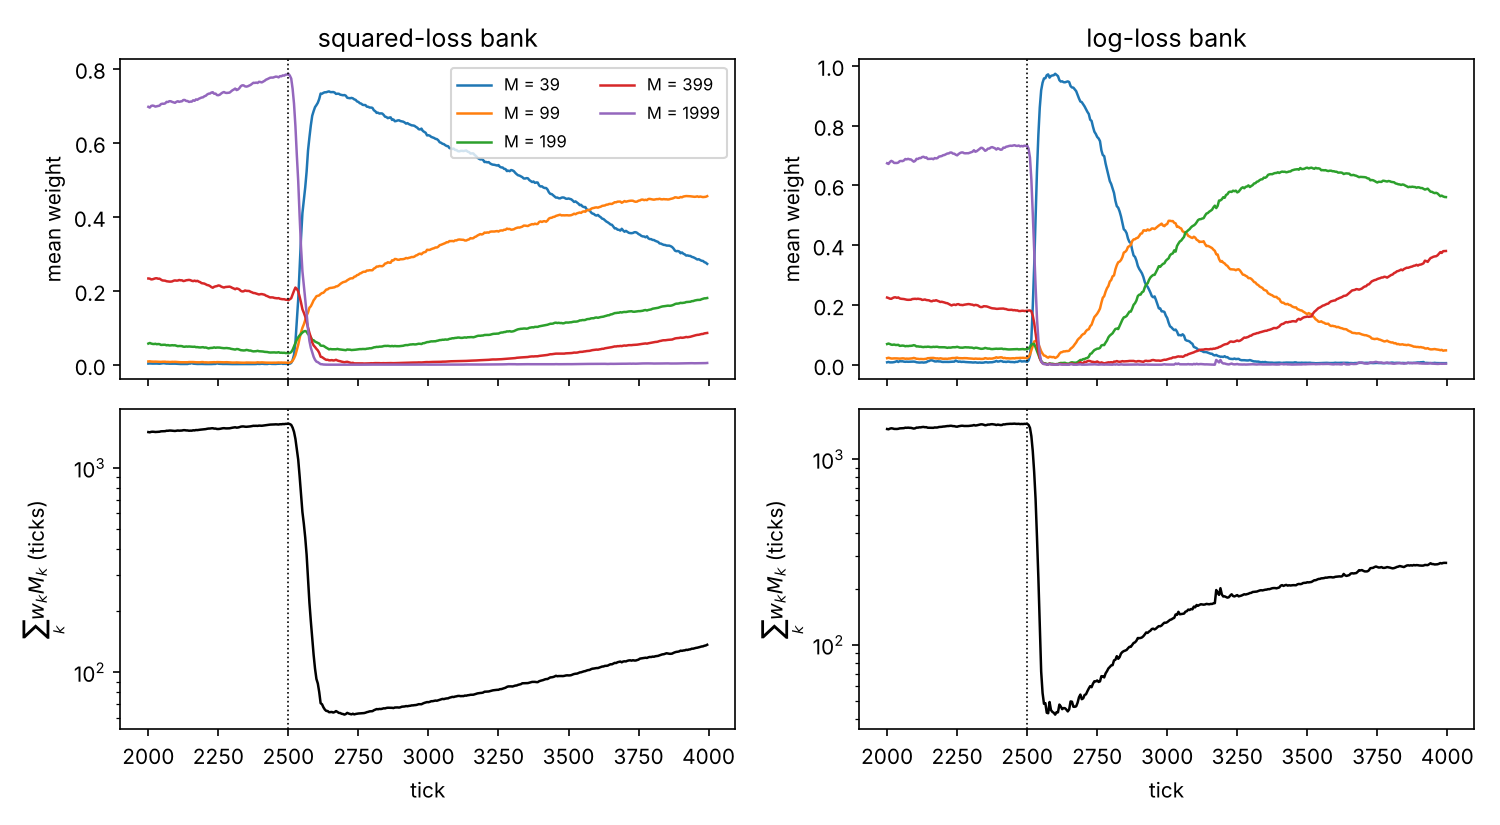
\includegraphics[width=\textwidth]{figures/ch6_bank_weights.png}
  \caption{Mean bank weights (top) and weight-averaged arm memory $\sum_k w_kM_k$ (bottom, log
    scale) around the jump at $t=2500$ (dotted). Gaussian copula, Xiao components, mean over 60
    seeds. Left: squared-loss bank; right: log-loss bank. The weight-averaged memory is a summary
    of where the weight sits, not an effective sample size.}
  \label{fig:weights}
\end{figure}

The VFF behaves differently. Its slow rate is the best method of all 500--1500 ticks after the
change ($25.6$), but it takes hundreds of ticks to get there, and its fast rate is unstable on
Gaussian data. On $t_4$ data, the fast VFF is the best method after the change
($53.1$ against $83.2$ for the log bank) but the worst before it ($154.4$ against $49.1$): it shortens
its memory in response to the heavier-tailed residuals of the $t$ copula even when the dependence
is not changing. A VFF tuned to react quickly also reacts to things that are not changes.

% -----------------------------------------------------------------------------
\section{Which loss to score with}
\label{sec:loss}

Section~5.3.1 argued that the squared and log losses agree to second order when the predictive
family is correct, and can disagree otherwise. Because every method here is scored on both
metrics, the experiment gives the full cross-classification of training loss against evaluation
metric (Table~\ref{tab:loss}).

\begin{table}[ht]
  \centering
  \caption{Log bank minus squared bank, Xiao components, whole run, mean $\pm2$\,SE over 60 seeds.
    Negative: the log bank is better. RMSE in $10^{-3}$; excess log loss in $10^{-3}$ nats per tick.}
  \label{tab:loss}
  \small
  \begin{tabular}{lrrrr}
    \toprule
    & \multicolumn{2}{c}{Gaussian} & \multicolumn{2}{c}{$t_4$} \\
    \cmidrule(lr){2-3}\cmidrule(lr){4-5}
    Scenario & RMSE & Excess log loss & RMSE & Excess log loss \\
    \midrule
    constant  & $-1.5\pm1.2$  & $-0.1\pm0.1$ & $+3.7\pm1.7$  & $+0.6\pm0.2$ \\
    drift     & $+0.2\pm0.4$  & $-0.1\pm0.1$ & $+2.8\pm0.7$  & $+0.5\pm0.1$ \\
    jump      & $-14.5\pm1.2$ & $-4.9\pm0.5$ & $-10.7\pm1.6$ & $-3.6\pm0.7$ \\
    oscillate & $+3.5\pm0.5$  & $+0.4\pm0.0$ & $+13.3\pm1.5$ & $+2.8\pm0.3$ \\
    \bottomrule
  \end{tabular}
\end{table}

Three things follow.

\emph{The two metrics rank the banks the same way.} In every row of Table~\ref{tab:loss}, and in
the full 48 cells (log bank better in 14 on RMSE and 15 on log loss), the sign of the RMSE
difference and the sign of the log-loss difference agree wherever both are distinguishable from
zero. With a Gaussian method-of-moments density the log loss is a function of
$\hat\rho^{(k)}$ alone, so this is expected: both losses measure how far each arm's $\rho$ is from
the data.

\emph{The log bank wins clearly on abrupt change and in every family.} On \emph{jump} it beats the
squared bank by $10.7$--$14.5\times10^{-3}$ in RMSE, including on the three families where its
Gaussian density is wrong.

\emph{When the family is wrong and the dependence is stationary or smooth, the log bank pays.} On
$t_4$ data it is worse than the squared bank on \emph{constant}, \emph{drift} and \emph{oscillate}.
The Gaussian density puts too little mass in the joint tails of a $t$ copula, so a $t$ observation
in the corner is penalised as if it were evidence against the current $\rho$, which favours the
short arms. The squared loss uses only the product $(\hat U_t-\tfrac12)(\hat V_t-\tfrac12)$ and is
not affected in the same way.

Two cautions. First, the two banks differ in $\eta$ and $\delta$ as well as in the loss
($\eta=0.5,\delta=10^{-4}$ against $\eta=1,\delta=4\times10^{-4}$), so the comparison is between two
configurations, not two losses \pending{rerun with $\eta,\delta$ tuned separately for each loss on
seeds 1--30, then report the same table}. Second, the excess log loss of every method on Clayton,
Gumbel and $t$ data contains a misspecification term of $30$--$80\times10^{-3}$ nats per tick, the
divergence between the true family and the Gaussian copula with the same $\rho_S$, which no memory
can remove. Differences in excess log loss between methods remain meaningful, but levels across
families are not comparable.

\pending{Planned refinement: score each estimator by its own predictive density (the MPL family
fit, or a family bank as in Section~\ref{sec:shape}), so that the log loss measures the copula and
not only $\rho$.}

% -----------------------------------------------------------------------------
\section{Changes in shape and tail dependence}
\label{sec:shape}

A change in the shape of the copula at constant $\rho_S$ is invisible to the squared loss by
construction: $\mathbb E[\hat p_t]$ does not move. This section collects the evidence on such
changes and on estimating tail dependence online. \pending{These results come from earlier probes
with a block-update bank and a histogram density (\texttt{memory\_tradeoff.md},
\texttt{tail\_dependence.md}); rerun with Algorithm~1 before submission.}

\paragraph{Shape switches.} In a Gaussian$\to t_4$ switch and a Clayton$\to$Gumbel switch at fixed
$\rho_S$, log-scored banks beat the best fixed memory over the whole run, by $3$--$9\times10^{-3}$
nats per tick. After Gaussian$\to t_4$ they stay ahead ($-7.9$ in the first 500 ticks). After
Clayton$\to$Gumbel they are worse in the first 500 ticks ($+3.1$ to $+4.5$), because before the
switch they had moved to memories of about 6000 ticks and so adapt more slowly than a fixed
1170-tick control. This is the shape-change analogue of the first 100 ticks in
Table~\ref{tab:recovery}.

\paragraph{Tail dependence needs longer memory than $\rho_S$.} The upper and lower tail coefficients
are estimated by the empirical $\chi(q)=P(U>1-q\mid V>1-q)$ at a finite threshold $q$. Two facts
measured on stationary streams shape what an online tail estimator can do:
\begin{itemize}
  \item The variance of $\hat\chi(q)$ from $M$ effective observations is close to
    $\chi(1-\chi)/(qM)$ (ratio measured at $0.89$--$1.08$ across families and thresholds): a tail
    estimator is a dependence estimator run on a stream thinned to rate $q$. At equal precision it
    therefore needs about $1/q$ times the memory of $\hat\rho_S$, and the bias--variance balance of
    Section~\ref{sec:fixed} puts its optimal memory correspondingly longer.
  \item The finite-threshold bias $\chi(q)-\lambda$ does not shrink with memory. A Gaussian copula,
    whose tail coefficient is zero, has $\chi(0.05)\approx0.31$. A Gaussian$\to t_4$ change in
    $\lambda_L$ from $0$ to $0.32$ is, at $q=0.05$, an observable change from $0.31$ to $0.41$.
\end{itemize}
Of the matched-$\rho_S$ transitions, Gaussian$\to t_4$ is the hardest to see in the tails: a
signal-to-noise ratio of 3 needs about 5000 ticks of memory, against 250--1000 ticks for transitions
involving Clayton or Gumbel.

\paragraph{Linking the bank to tail dependence.} Two extensions follow directly from
Algorithm~1, and are the natural next experiments \pending{not yet run}:
\begin{enumerate}
  \item \emph{A bank over families.} Replace the five memories of one estimator with online MPL
    fits of several families (Gaussian, Clayton, Gumbel, $t_4$) and score them by log loss. The
    bank's implied tail coefficient is then $\hat\lambda_t=\sum_kw_{k,t}\lambda(\hat\theta_{k,t})$,
    and its weights become an online measure of which tail shape the data support.
  \item \emph{A bank over memories for $\hat\chi(q)$.} Apply Algorithm~1 to $\hat\chi(q)$ at several
    memories, scored on tail exceedances, for example with the censored log score of Diks,
    Panchenko and van Dijk (2011). Because of the $1/(qM)$ variance, its arms should be
    about $1/q$ times longer than those used for $\rho_S$.
\end{enumerate}
A useful ceiling for both is the known-changepoint ``soft restart'', which at a change keeps a
fraction $\gamma^*=1/(1+Z^2)$ of the old evidence, $Z$ being the standardised size of the change.
An online method that does not know the change point can at best approach it.

% -----------------------------------------------------------------------------
\section{Computational cost}
\label{sec:cost}

Every method is single pass with bounded state. Table~\ref{tab:cost} gives the state of one
estimator and of the corresponding bank, measured with each object's own byte count, and the
wall-clock time per tick on one core.

\begin{table}[ht]
  \centering
  \caption{State size and time per tick, measured over a 200\,000-tick stream. Times are
    indicative (single run, shared cloud machine).}
  \label{tab:cost}
  \begin{tabular}{lrrrr}
    \toprule
    & \multicolumn{2}{c}{Single estimator} & \multicolumn{2}{c}{Bank, $K=5$} \\
    \cmidrule(lr){2-3}\cmidrule(lr){4-5}
    Estimator & bytes & ns/tick & bytes & ns/tick \\
    \midrule
    Xiao ($20\times20$)  & 3\,824  & 650 & 35\,672 & 6\,000--7\,000 \\
    Hermite ($N=10$)     & 1\,192  & 580 & 22\,512 & 5\,100--5\,700 \\
    MPL, Gaussian        & 16\,400 & 540 & 18\,712 & 1\,600--2\,000 \\
    Xiao VFF             & 19\,968 & 1\,500 & & \\
    \bottomrule
  \end{tabular}
\end{table}

The bank's state is the $K$ arms plus the two shared rank windows ($2\times500$ values, about
16\,kB), and its time per tick is about $K$ times that of one arm, plus $O(K)$ for the weights. The
stand-alone MPL figure is dominated by its own rank window; inside the bank that window is shared,
which is why the MPL bank is barely larger than one MPL estimator. All of these are constant in the
length of the stream: at about $5\,\mu$s per tick the most expensive bank processes some 200\,000
pairs per second on one core.

% -----------------------------------------------------------------------------
\section{Summary of findings}
\label{sec:summary}

\begin{enumerate}
  \item \emph{Memory is the first-order design choice.} The best fixed memory ranges from about 36
    ticks to more than 30\,000 across the scenarios, and choosing it changes RMSE by a factor of 2 to
    17; choosing between estimators at the same memory changes it by 3--15\%.
  \item \emph{The bank removes the need to know the memory in advance.} It beats any single memory
    chosen in advance in every scenario, family and estimator, and on an abrupt change it beats
    even the best memory chosen in hindsight (log bank: $15$--$21\times10^{-3}$ in RMSE).
  \item \emph{The price is a few $10^{-3}$ when the right memory is fixed}, mainly from the fixed
    share, and a slow first 100 ticks after a change, while the bank gathers evidence.
  \item \emph{Choosing beats averaging.} Uniform weights over the same arms are worse than the bank
    in 46 of 48 cells and tie in the other two.
  \item \emph{Against variable forgetting factors}, the bank is better in 41 of 48 cells in RMSE.
    The one VFF rule that adapts (Xiao's) is better on stationary and slowly drifting dependence,
    and worse on abrupt and periodic change. The other two rules are inert or unstable as tuned,
    and these conclusions apply to these rules only.
  \item \emph{Log loss helps on abrupt change and hurts under misspecification.} With a Gaussian
    scoring density, the log bank is best on jumps in every family, and worse than the squared bank
    on stationary $t_4$ data.
  \item \emph{Tail dependence needs a different memory.} Tail estimators behave like dependence
    estimators on a stream thinned by $q$, so a bank for tail dependence needs longer arms; this,
    and a bank over families, are the extensions left for future work.
\end{enumerate}
\pending{Revisit items 2, 3 and 6 after $\eta,\delta$ are tuned on separate seeds.}
